\documentclass[12pt]{article}

\usepackage{fancyhdr}
\usepackage{amsthm}
\usepackage{amsmath}
\usepackage{graphicx}
\usepackage{amssymb}
\usepackage{esint}
\usepackage{subfigure}
\usepackage{color}
\usepackage{moreverb}
\usepackage{wrapfig}
\usepackage{subfig}

\textwidth 17cm \topmargin -1cm \oddsidemargin 0cm \textheight 21.5cm
\pagestyle{empty} \pagestyle{fancyplain}
\lhead[\fancyplain{}{}]{\fancyplain{}{{\sc Myles Adams}}}
\chead[\fancyplain{}{}]{\fancyplain{}{{\sc CS 111 Final}}}
\rhead[\fancyplain{}{}]{\fancyplain{}{{\sc Fall 2017}}}

\newcommand{\etal}{\textit{et al. }}

\begin{document}
\centerline{\Large\textbf{CS 111 Final}}
\vspace{.5cm}

\section*{Introduction}\label{sec::Intro}
\section*{Problem 1}\label{sec::Problem1}
\subsection*{Part A}
\subsection*{Part B}
\subsection*{Part C}

\begin{figure}[htb]%
    \centering
    {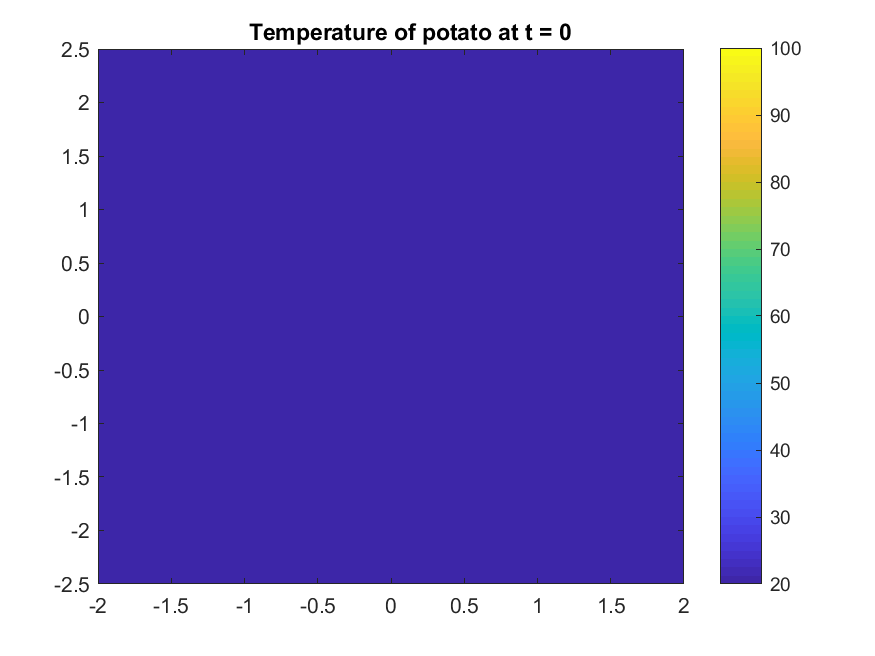
\includegraphics[width=8cm]{Problem1_fig1.png}}%
    \qquad
    {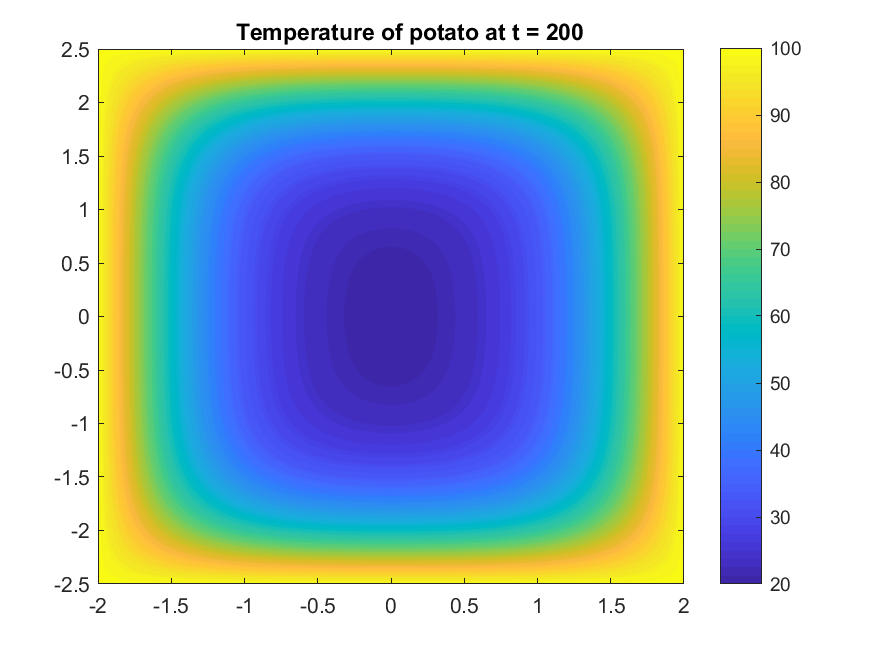
\includegraphics[width=8cm]{Problem1_fig2.png}}%
    \label{fig:fig1 and fig2}%
\end{figure}

\begin{figure}[htb]%
    \centering
    {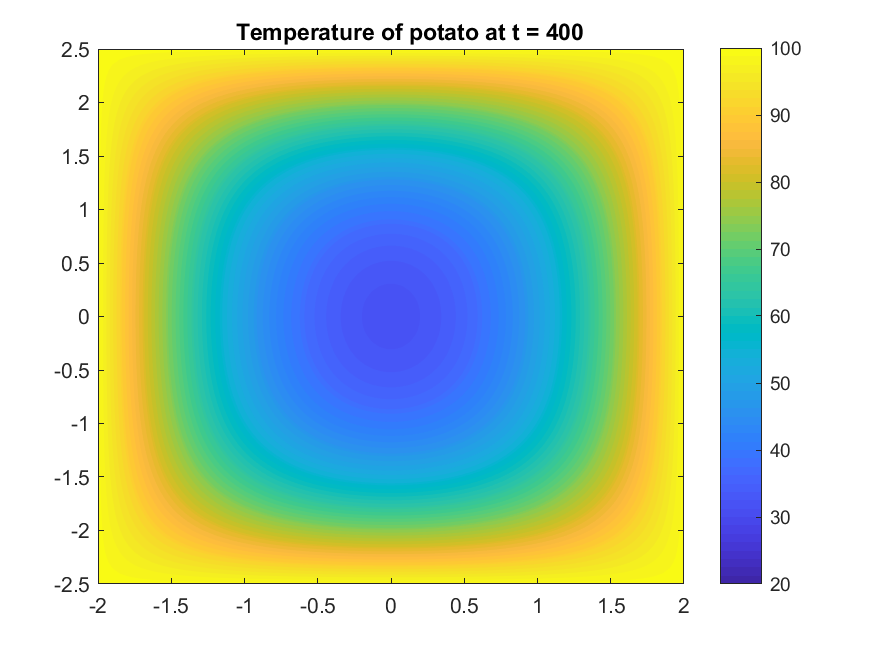
\includegraphics[width=8cm]{Problem1_fig3.png}}%
    \qquad
    {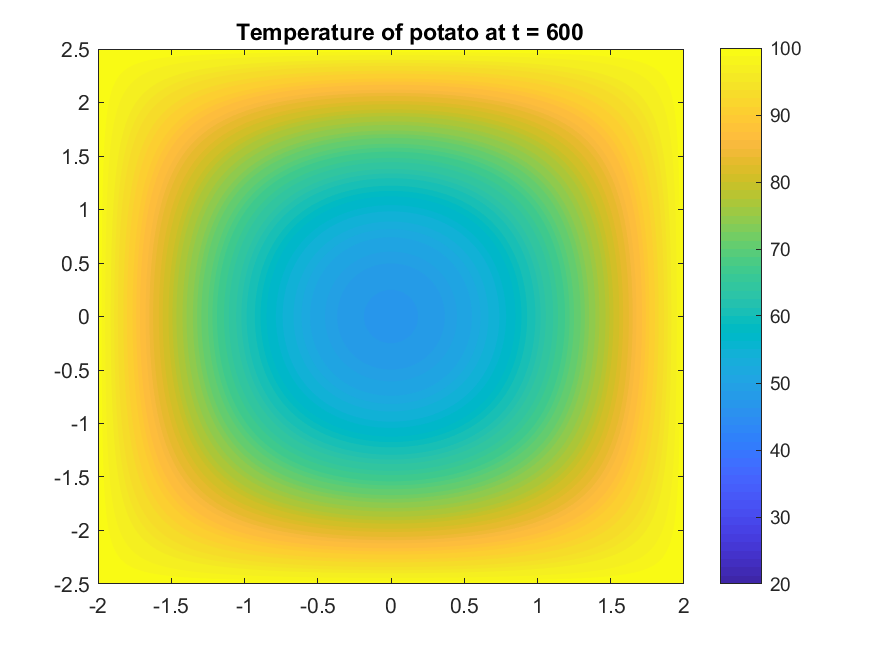
\includegraphics[width=8cm]{Problem1_fig4.png}}%
    \label{fig:fig3 and fig4}%
    \caption*{Temperature ($^{\circ}$C) throughout the potato at various times}
\end{figure}

\begin{figure}[htb]
\centering
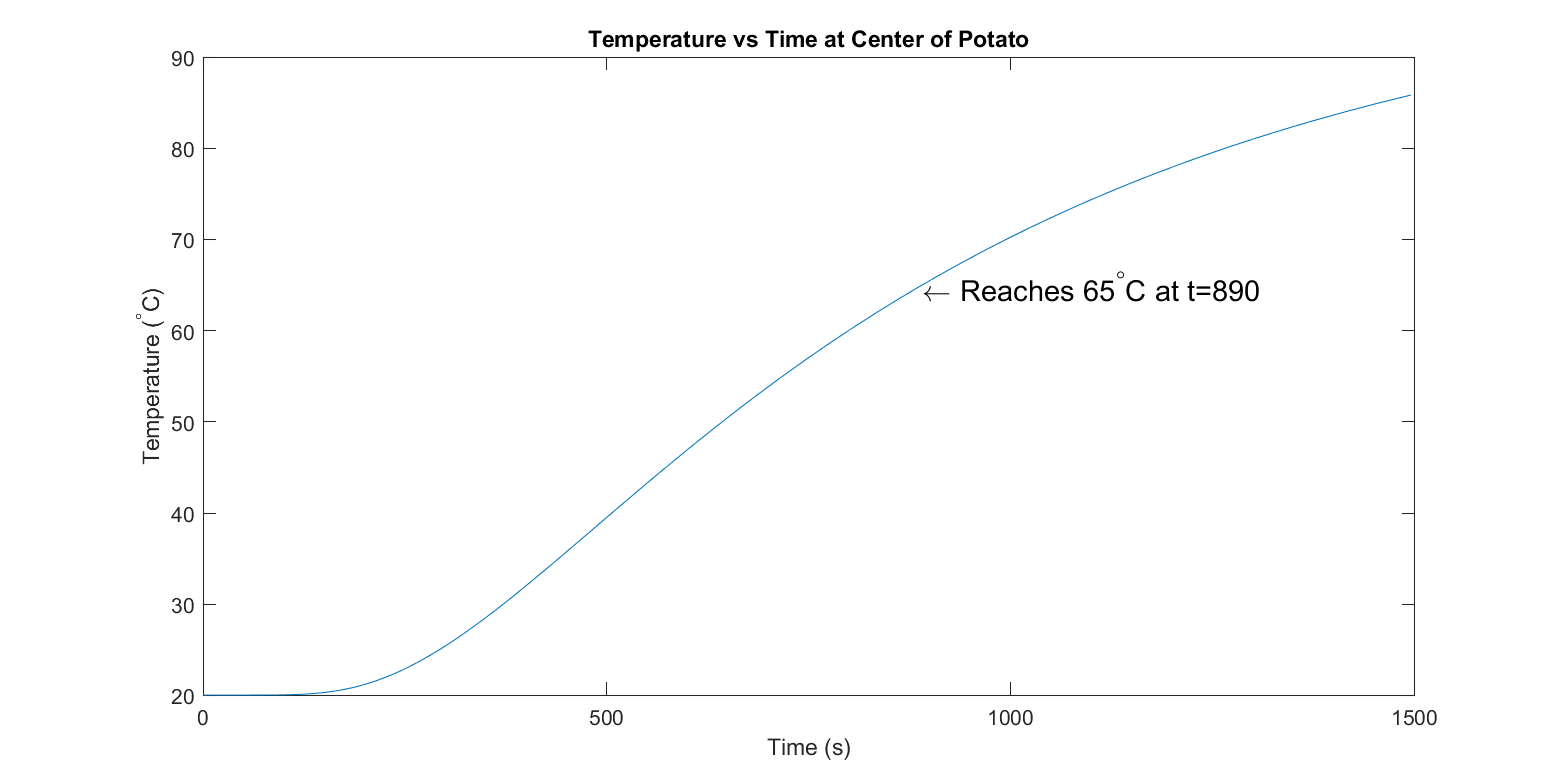
\includegraphics[width=1\textwidth]{Problem1_fig5.png}
\caption*{Temperature ($^{\circ}$C) at the center of potato vs time}
\label{fig::fig5}
\end{figure}

\section*{Problem 2}\label{sec::Problem2}
\subsection*{Part A}
\subsection*{Part B}
\subsection*{Part C}

\newpage
\clearpage
\setcounter{page}{1} \pagestyle{empty}
\section*{References}\label{sec::References}
\begin{itemize}
\item [1] Daniil Bochkov, CS 111 - Introduction to Computational Science - Midterm, Fall 2017
\item [2] Daniil Bochkov, CS 111 - Introduction to Computational Science - Lecture 4 - High-Order Methods, Fall 2017
\item [3] Daniil Bochkov, CS 111 - Introduction to Computational Science - Lecture 6 - Systems of ODEs,  Fall 2017
\item [4] Daniil Bochkov, CS 111 - Introduction to Computational Science - Lecture 7 - High-Order ODEs, Fall 2017
\end{itemize}
\end{document}
